\documentclass[12pt]{article}
\usepackage[utf8]{inputenc}
\usepackage[french]{babel}
\usepackage{amsmath,amsthm,amsfonts,amssymb}
\usepackage{lmodern}
\usepackage[top=2.4cm,bottom=2.4cm,left=2cm,right=2cm]{geometry}
\usepackage{hyperref}
\usepackage{multicol}
\usepackage{enumitem}
\usepackage{listings}
\usepackage[dvipsnames]{xcolor}
\usepackage{tikz}

%\date{}
\title{{\bf  Génie logiciel} \\
	Notes du cours de 02/12  \\
	{\small L3 Informatique appliquée 2022-2023} \\
	{\it \small MABROUK Fayez}}
\begin{document}
	\maketitle
	\newpage
		\section{UML pour modéliser la structure}
	\subsection{Héritage}
	\begin{itemize}
		\item[* ] Les instances d'une sous-classe sont également des instances de la
		superclasse.
		\item[* ] Par conséquent, elles héritent des méthodes définies dans la
		superclasse.
		\item[* ] Exemple:
		\begin{figure}[!hbtp]
			\centering
			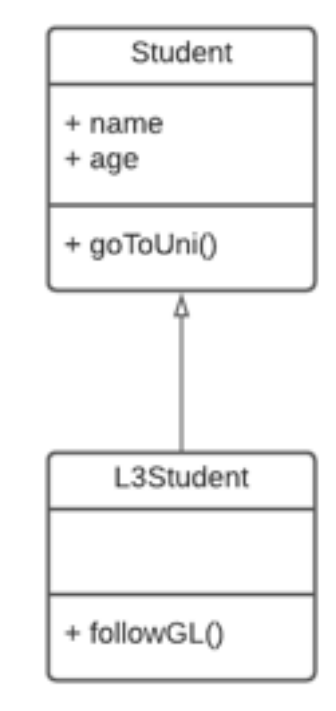
\includegraphics[scale=0.75]{Capture1.PNG}
			%\caption{Légende de l'image}
		\end{figure}
	\item[* ] Notez que vous pouvez explicitement montrer des éléments hérités
	en les préfixant avec "chapeau".
	\item[* ] Enfin, notez que les associations entre une classe et une
	superclasse est héritée par ses sous-classes.
		\begin{figure}[!hbtp]
		\centering
		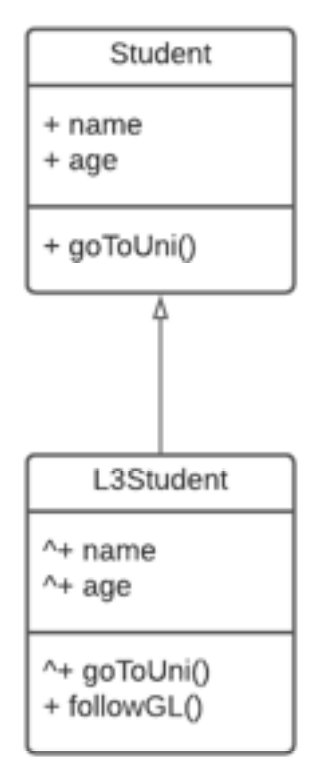
\includegraphics[scale=0.75]{Capture2.PNG}
		%\caption{Légende de l'image}
	\end{figure}
	\end{itemize}
	\subsection{Héritage multiple}
	\begin{itemize}
		\item[* ] Il est possible qu'une classe soit une spécialisation de plus d'une classe.
		\item[* ] Exemple : La classe C est une spécialisation de la classe A et de la classe B.
			\begin{figure}[!hbtp]
			\centering
			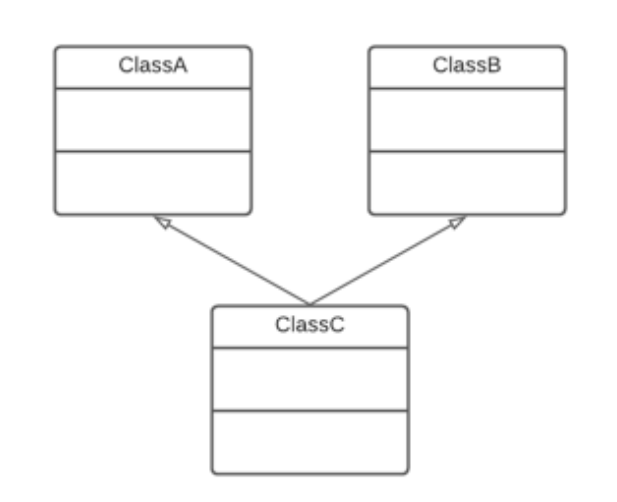
\includegraphics[scale=0.75]{Capture3.PNG}
			%\caption{Légende de l'image}
		\end{figure}
	\item[* ] L'héritage multiple peut être problématique si un attribut de même nom/type ou un
	nom/type ou un code mathématique avec la même signature est défini dans plus d'une superclasse.
	une superclasse.
	\item[* ] Pas toujours possible en pratique : pas d'héritage multiple en Java.
	
	\end{itemize}
	\subsection{Contraintes}
	\begin{itemize}
		\item[* ] Il est possible d'ajouter des contraintes sur la relation, soit
		sur :
		\begin{itemize}
			\item[* ] la complétude : la spécialisation peut être complète ou
			incomplète. Si elle est complète, elle indique que l'ensemble des
			domaines des sous-classes couvre le domaine de la super-classe.
			\item[* ] superposition : la spécialisation peut être soit disjointe (elle n'a pas d'instances communes), soit superposée.
			n'ont pas d'instances communes) ou superposées (elles peuvent avoir des
			instances communes)
			
		\end{itemize}
	\item[* ] Syntaxe : {contrainte}.
	\newpage
	\item[* ] Exemple:
		\begin{figure}[!hbtp]
		\centering
		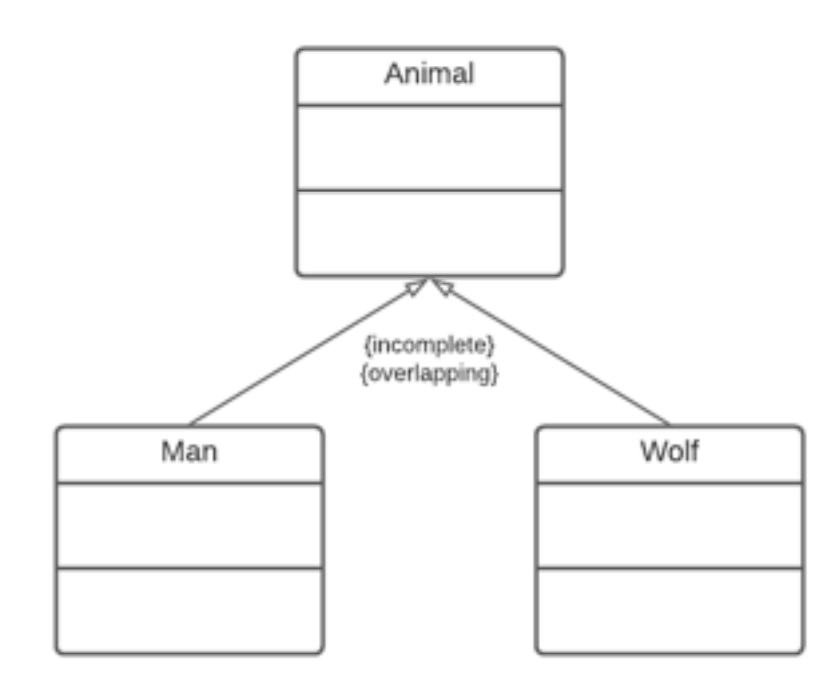
\includegraphics[scale=0.75]{Capture4.PNG}
		%\caption{Légende de l'image}
	\end{figure}
	\item[* ] il y a d'autres animaux que les hommes
	et les loups, donc la relation est
	incomplète
	\item[* ] si vous croyez aux loups-garous, une
	instance peut être à la fois un homme et un
	loup, donc la relation se chevauche.
	\begin{figure}[!hbtp]
		\centering
		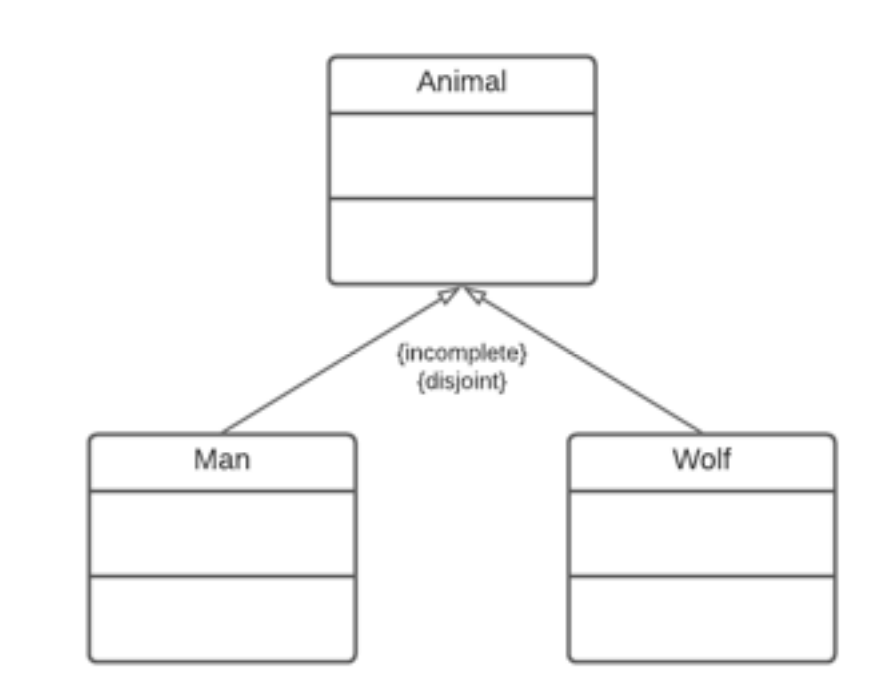
\includegraphics[scale=0.75]{Capture5.PNG}
		%\caption{Légende de l'image}
	\end{figure}
	\item[*] Probablement, un homme ne peut pas être un loup.
	\end{itemize}
	\subsection{Stéréotypes}
	\begin{itemize}
		\item[* ] Les stéréotypes peuvent être utilisés pour spécialiser un élément en UML.
		\item[* ] Syntaxe : <<stéréotype>> au-dessus du nom de la classe.
		\newpage
		\begin{figure}[!hbtp]
			\centering
			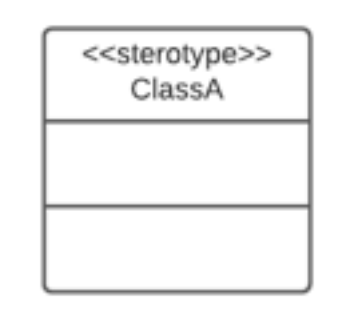
\includegraphics[scale=0.75]{Capture6.PNG}
			%\caption{Légende de l'image}
		\end{figure}
	\item[* ] Stéréotypes possibles :
	\begin{itemize}
		\item[* ] énumération : classe présentant un type avec une liste de valeurs constantes.
		\item[* ] auxiliaire : pour indiquer une classe secondaire.
		\item[* ] abstrait.
		\item[* ] interface.
	\end{itemize}
	\end{itemize}
	\subsection{Abstract classes}
	\begin{itemize}
		\item[* ] Rappel : Abstrait et concret
		classes abstraites : les classes abstraites sont des classes qui
		n'ont pas d'instances (par exemple Mammal).
		Les classes concrètes en ont (par exemple Human).
		\item[* ] Les classes abstraites permettent de hiérarchiser les classes
		de classes et de regrouper les attributs et les
		méthodes. Elles doivent avoir des sous-classes.
		\item[* ] Exemple : la méthode communicate de
		classe Animal est abstraite (indiquée en
		italique). Elle n'est pas définie pour un animal,
		mais elle l'est pour les classes concrètes.
		\item[* ]  Note : peut aussi être indiquée en italique
		le nom de la classe.
			\begin{figure}[!hbtp]
			\centering
			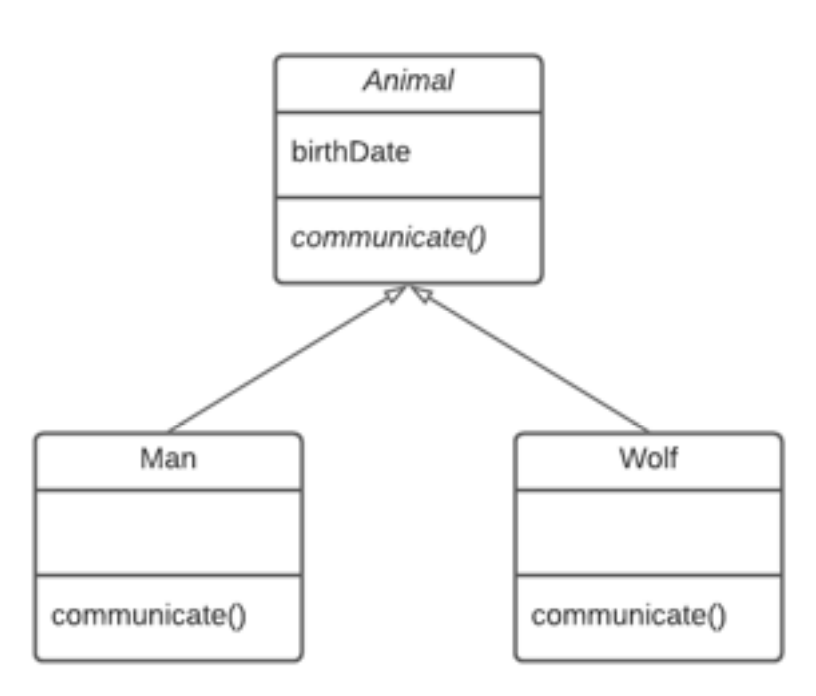
\includegraphics[scale=0.75]{Capture7.PNG}
			%\caption{Légende de l'image}
		\end{figure}
	\end{itemize}
	\subsection{Interface}
	\begin{itemize}
		\item[* ] Définition : une interface est une classe totalement abstraite : elle ne possède aucun attribut et ses méthodes sont toutes publiques.
		n'a aucun attribut et ses méthodes sont toutes publiques et abstraites.
		et abstraites.
		\newpage
		\item[* ] Syntaxe : stéréotype + flèche vide en pointillés.
			\begin{figure}[!hbtp]
			\centering
			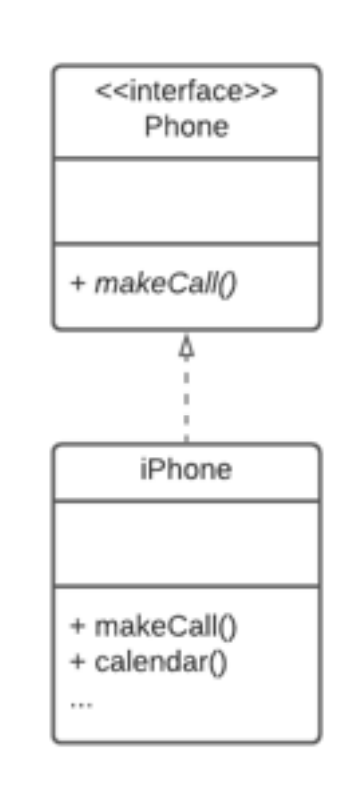
\includegraphics[scale=0.75]{Capture8.PNG}
			%\caption{Légende de l'image}
		\end{figure}
	\item[* ] Alternative : sucette.
	\begin{figure}[!hbtp]
		\centering
		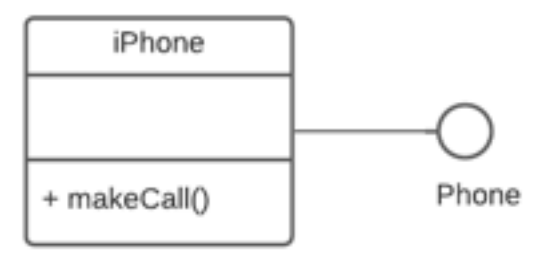
\includegraphics[scale=0.75]{Capture9.PNG}
		%\caption{Légende de l'image}
	\end{figure}
\item[* ] Lorsqu'il y a une dépendance sur une interface, on peut être
notée "classiquement".
\begin{figure}[!hbtp]
	\centering
	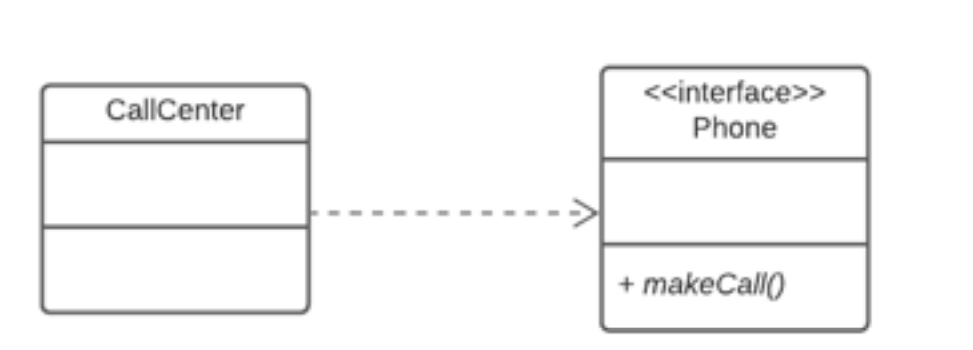
\includegraphics[scale=0.75]{Capture10.PNG}
	%\caption{Légende de l'image}
\end{figure}
\item[* ] Ou à travers une sucette(a lollipop).
\begin{figure}[!hbtp]
	\centering
	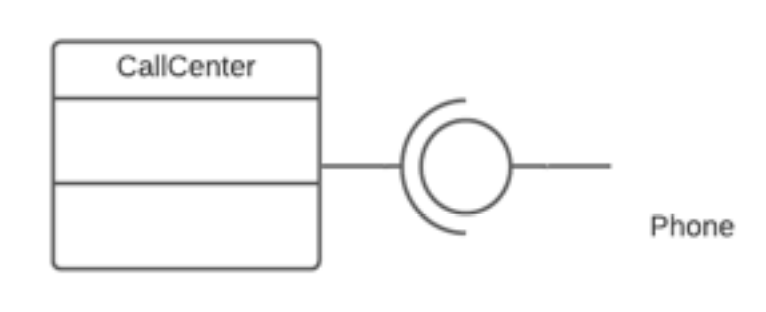
\includegraphics[scale=0.75]{Capture11.PNG}
	%\caption{Légende de l'image}
\end{figure}
	\end{itemize}
	\subsection{Représentation d'un objet}
	\begin{itemize}
		\item[* ] Le diagramme de classes représente une vue statique de la structure.
		\item[* ] Le diagramme d'objets peut montrer un instantané du système :
		\item[* ] Le diagramme d'objets montre les instances et les valeurs de leurs attributs.
		\item[* ] Syntaxe : nom de l'instance:nom de la classe.
		\begin{figure}[!hbtp]
			\centering
			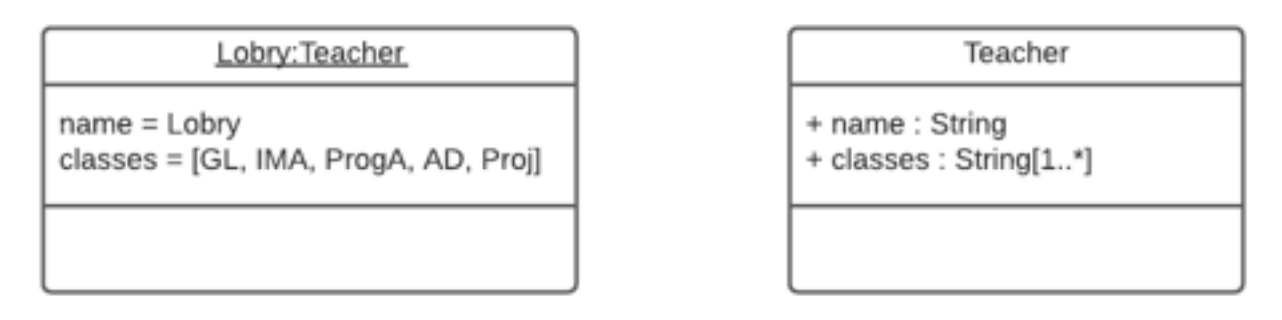
\includegraphics[scale=0.75]{Capture12.PNG}
			%\caption{Légende de l'image}
		\end{figure}
	\item[* ] Lien "instanceOf" facultatif.
	\begin{figure}[!hbtp]
		\centering
		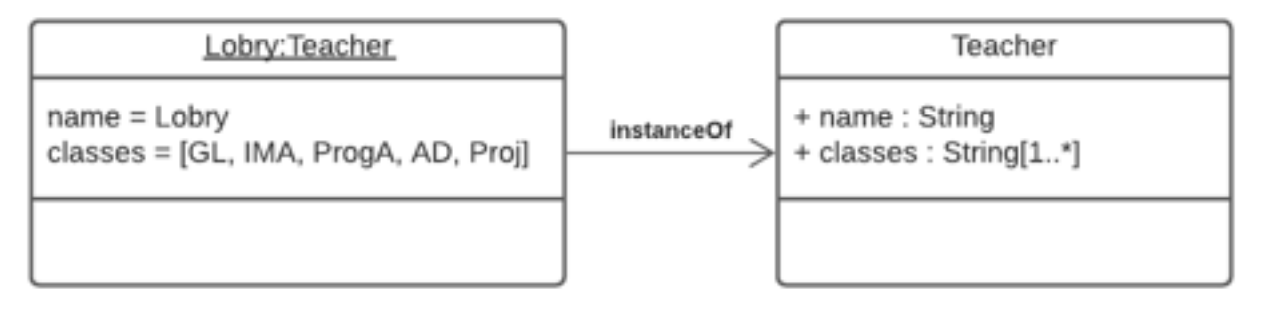
\includegraphics[scale=0.75]{Capture13.PNG}
		%\caption{Légende de l'image}
	\end{figure}
	\end{itemize}
\subsection{Relation entre les instances}
\begin{itemize}
	\item[* ] Enfin, il est possible de représenter
	les interactions entre les instances
	avec une ligne pleine.
	\item[* ] Facultatif : nom de la relation et
	rôles.\\
	\begin{figure}[!hbtp]
		\centering
		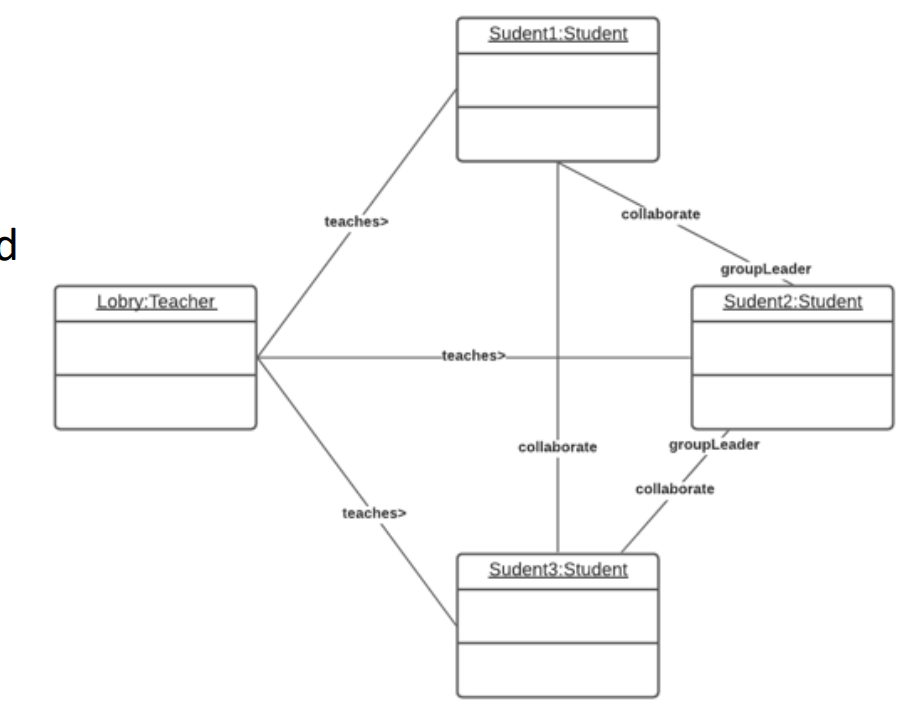
\includegraphics[scale=0.75]{Capture14.PNG}
		%\caption{Légende de l'image}
	\end{figure}
\end{itemize}
\subsection{Conclusion}
\begin{itemize}
	\item[* ]  Les diagrammes de classes permettent d'ajouter des informations sur la structure de notre modèle.
	\item[* ] L'ajout des bons liens entre les classes améliore la sémantique et rend le
	diagramme plus léger.
	\item[* ] Comme toujours avec la modélisation :
	\begin{itemize}
		\item[* ] Faites attention à la cible du modèle : qu'ont-ils besoin de savoir ?
		\item[* ] Pas seulement un diagramme, il doit être accompagné d'une documentation (en particulier : vos choix)
		\item[* ] Pas une bonne solution unique.
	\end{itemize}
\item[* ] Nécessite de la pratique.
\end{itemize}
\end{document}